\documentclass[12pt]{article}
\usepackage{graphicx}
\begin {document}
\section{Estimating long-term multivariate progression from short-term data}


\subsection{Introducción}
En este texto, centrado en un planteamiento de la enfermedad del Alzheimer (EA), se observa lo complejo que es el estudio del desarrollo de las enfermedades crónicas. Una de las dificultades principales es establecer un punto de inicio claro para el modelo de la progresión de la enfermedad. Esto se debe a la observación de grupos de personas en diferentes etapas de la enfermedad,  a través de "instantáneas" longitudinales a corto plazo. Además, es fundamental la utilización de biomarcadores y datos cognitivos para entender la progresión de la EA incluso antes de que aparezcan síntomas claros.\\

Por otra parte, se presenta el modelo SEMOR (Self-modeling regresión), el cual estima a largo plazo las trayectorias del Alzheimer y otros resultados aun teniendo un conjunto limitado de datos a lo largo del tiempo. Es de gran importancia modelar curvas de progresión a largo plazo en función de múltiples medidas,ya que permite ver los cambios de los pacientes según su desempeño en las distintas evaluaciones. A parte, se habla del estudio "Personnes Agées Quid" (PAQUID) que proporciona trayectorias a largo plazo del Examen del Estado Mental Mínimo (MMSE). Esta información servirá como complemento de los datos de la ADNI para comprender mejor la progresión de la EA.

\subsection{Modelo}
El modelo propone que varios resultados $Y_{ij}$ ocurren durante un tiempo \textit{t} para individuos \textit{i=1,...,n} y marcadores \textit{j=1,...,m} según la ecuación:
\begin{center}
	$Y_{ij}(t)=g_{j}(t+\gamma_{i})+\alpha_{0ij}+\alpha_{1ij}t+\epsilon_{ij}(t)$
\end{center}

Cada $g_{j}$ es una función monótona continuamente diferenciable con media cero y varianza $\sigma_{\gamma}^{2}$. Las tuplas $(\alpha_{0ij},\alpha_{1ij})$ siguen una distribución gaussiana con media cero y matriz de covarianza $\sum_{j}$. Los errores residuales $\epsilon_{ij}(t)$ son gaussianos e independientes con media cero y una variación específica para cada marcador.

El "tiempo de observación a corto plazo" se representa mediante la covariable observada \textit{t}, mientras que el "tiempo de progresión a largo plazo" se representa por \textit{t+$g_{i}$}, donde $g_{i}$ es el desplazamiento temporal específico del sujeto. El objetivo del algoritmo es estimar tanto los parámetros temporales como las curvas a largo plazo, asumiendo que estas son monótonas y utilizando la información entre los marcadores para estimar desplazamientos temporales específicos. Este modelo es una versión simplificada del modelo SIM clásico para cada marcador, excluyendo los parámetros de reescalado pero incluyendo una pendiente adicional aleatoria.

\subsection{Algoritmo}
Para abordar la complejidad del problema multidimensional, se desglosará en etapas con el algoritmo. Para ello se estiman los parámetros desconocidos $(g_{j}, \gamma_{i}$ y $\alpha)$ de forma secuencial, utilizando las estimaciones actuales de los otros parámetros en cada iteración hasta alcanzar la convergencia del error cuadrático (RSS). Para lograrlo, se utilizan tres tipos de residuos parciales, cada uno proporcionando una estimación imparcial de un parámetro desconocido, siempre que el modelo inicial sea correcto.\\

Tras inicializar $\gamma_{i}$ a cero, comienza el proceso que se dividirá en dos etapas principales:
\begin{description}
	\item {\textbf{Etapa 1}} Estimación de funciones monótonas y parámetros específicos para cada marcador \textit{j}
	
	Se inicia estimando las funciones monótonas $g_{j}$	y los parámetros específicos para cada marcador. Para cada \textit{j}, se utilizan subrutinas paralelas para ajustar $g_{j}$
	y los parámetros $\alpha_{0ij}$ y $\alpha_{1ij}$ específicos, utilizando un suavizado monótono y un modelo lineal mixto, respectivamente.
	\item {\textbf{Etapa 2}} Estimación de desplazamientos temporales $\gamma_{i}$
	
	Se invierten las variables y se estima el desplazamiento temporal $\gamma_{i}$ promediando los residuos de todos los marcadores y tiempos para cada individuo. Este paso es fundamental para lograr la convergencia del error cuadrático total.
\end{description}

El algoritmo se repite iterativamente hasta que se alcanza la convergencia deseada, logrando estimaciones precisas y refinadas de los parámetros y curvas de interés para abordar el problema complejo en estudio.
		
\subsection{Simulaciones}
Mediante el algoritmo diseñado en el apartado anterior, se simularon los datos del modelo y se estimaron curvas utilizando un suavizante monótono de B-spline con cinco nudos equiespaciados y splines polinómicos de quinto grado. En las imágenes siguientes, se ve como las curvas ajustadas resultantes demostraron una alta precisión al replicar las curvas logísticas, lineales y cuadráticas verdaderas .\\

Además, se compararon los desplazamientos temporales reales con los estimados a partir de la simulación, aunque esta comparación no se muestra visualmente. A pesar de que no hubo una concordancia perfecta, la línea de regresión en el gráfico de dispersión estuvo cercana a la línea de identidad, como se anticipaba. El error cuadrático residual (RSS) para cada marcador convergió en 10 iteraciones, alcanzando una tolerancia del 0.1\% del RSS.

\subsection{Resultados ADNI y PAQUID}

El texto explora los resultados basados en datos recopilados durante el Alzheimer's Disease Neuroimaging Initiative (ADNI) y el estudio Personnes Agées Quid (PAQUID). El objetivo principal es comprender la progresión de la enfermedad de Alzheimer (AD) a través de un análisis detallado de diversos marcadores clave. Se busca derivar curvas de progresión basadas en datos reales, alejándose de las hipótesis teóricas.\\

El proceso comienza con la transformación de los datos a una escala percentil. Esta transformación facilita la comparación significativa entre grupos heterogéneos, permitiendo un análisis más profundo de la progresión de la enfermedad. Se exploran trayectorias de progresión en diferentes grupos, incluidos aquellos con acumulación de amiloide y portadores de ciertos alelos genéticos. En la \ref{fig:figura1} se visualiza la progresión a lo largo del tiempo de distintos marcadores como la acumulación de amiloide en los distintos grupos.\\

\begin{figure}[h!]
	\centering
	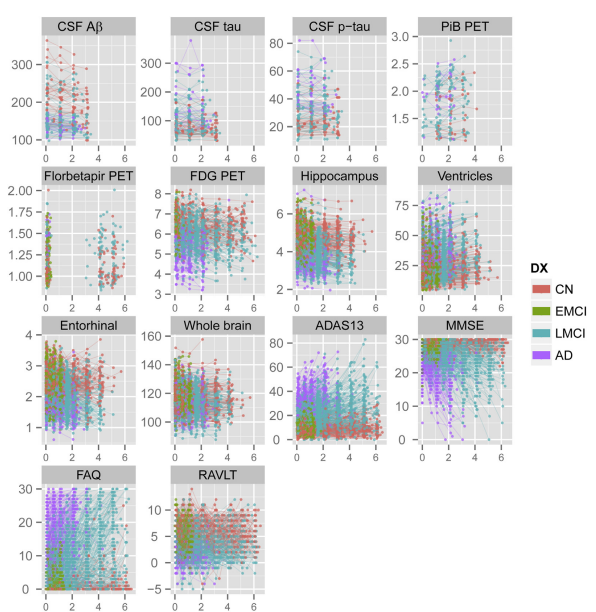
\includegraphics{fig.1}
	\caption{}
	\label{fig:figura1}
\end{figure}

Se destaca la asociación entre la acumulación de placas de amiloide en el cerebro y la disminución del líquido cefalorraquídeo (CSF), junto con un aumento en la captación de PiB y florbetapir en la tomografía por emisión de positrones (PET). Se utiliza un enfoque de suavizado basado en B-spline para estimar las curvas de progresión a largo plazo, brindando una visualización clara de la evolución de la enfermedad en diferentes cohortes.\\

El estudio también investiga subgrupos de sujetos, incluyendo aquellos con evidencia de acumulación de amiloide y portadores del alelo $\epsilon$4 de la apolipoproteína E (APOE). En \ref{fig:figura2} se presentan las trayectorias estimadas de dos grupos: aquellos sin evidencia de carga amiloide y aquellos sin el alelo $\epsilon$4 de APOE.\\

\begin{figure}[h!]
	\centering
	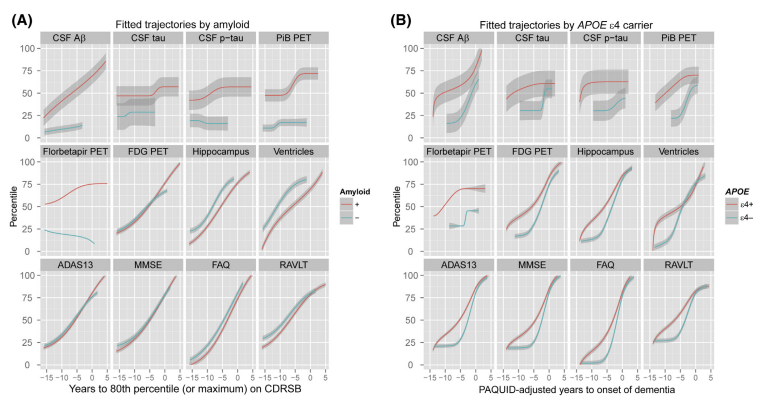
\includegraphics{fig.2}
	\caption{}
	\label{fig:figura2}	
\end{figure}


Se observa que los portadores de este alelo tienen una progresión más rápida de la enfermedad en comparación con los no portadores. Se emplea una transformación del tiempo para comparar las trayectorias de progresión con el estudio PAQUID, proporcionando información valiosa sobre la relación entre la carga de amiloide, la genética y la progresión clínica. 


\subsection{Discusión}
El texto examina la forma en que se analiza la evolución de la enfermedad de Alzheimer, utilizando datos de dos estudios: el Alzheimer's Disease Neuroimaging Initiative (ADNI) y el estudio Personnes Agées Quid (PAQUID). Se compara este enfoque con un estudio previo que se centró en cómo se hereda la enfermedad de Alzheimer, utilizando la edad en la que los padres desarrollaron síntomas para estimar la progresión de la enfermedad. Sin embargo, en este estudio, se aborda una limitación importante de ADNI al estimar tanto la edad en que se desarrollan los síntomas como las formas de evolución de la enfermedad al mismo tiempo.

Además, se resaltan las diferencias en las curvas de evolución de diversos marcadores de la enfermedad, como los niveles de proteína beta-amiloide en el líquido cefalorraquídeo (CSF), la proteína tau, los resultados de tomografía por emisión de positrones (PET) con el compuesto Pittsburgh Compound B (PiB), el metabolismo de la glucosa y el tamaño del hipocampo. Se sugiere que estos marcadores siguen trayectorias distintas y que algunos tienen una evolución más constante, mientras que otros muestran un patrón de crecimiento y descenso.

Por otra parte, se menciona la influencia de factores como la genética, la dieta y el estilo de vida en la variabilidad de los marcadores de la enfermedad. Se subraya la necesidad de incluir datos de grupos de estudio más jóvenes y se argumenta que la combinación de datos de múltiples fuentes ayudará a validar modelos de progresión de la enfermedad de Alzheimer en el futuro.


\end{document}